\chapter{Implementation details}
The programming language used for developing the tool is \textit{\textbf{Python}} . Python is a general-purpose interpreted, object-oriented, and high-level programming language. It was created by Guido van Rossum during 1985- 1990. \cite{python}
In addition \textit{\textbf{PyQt}} is used as UI layer. PyQt is a Python binding for the Qt cross-platform C++ framework. 

\section{Processing phases}
\tab In order to build structural and logical dependencies the tool that takes as input the source code repository and builds the required software dependencies . The workflow can be delimited by three major steps as it follows  (Figure \ref{fig:fig3}):  \\\\
\textit{\textbf{Step 1:} Extracting structural dependencies.}\\
\textit{\textbf{Step 2:} Extracting logical dependencies.}\\
\textit{\textbf{Step 3:} Processing the information extracted and graphics generation.}

\begin{figure}[h]
\centering
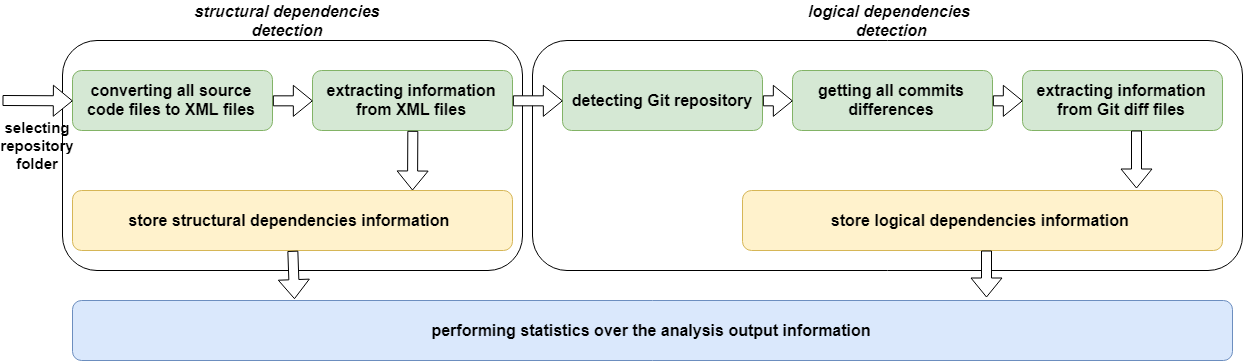
\includegraphics[width=\textwidth]{fig3.png}
\caption{Processing phases}
\label{fig:fig3}
\end{figure}


\section{Architecture}

\begin{figure}[h]
\centering
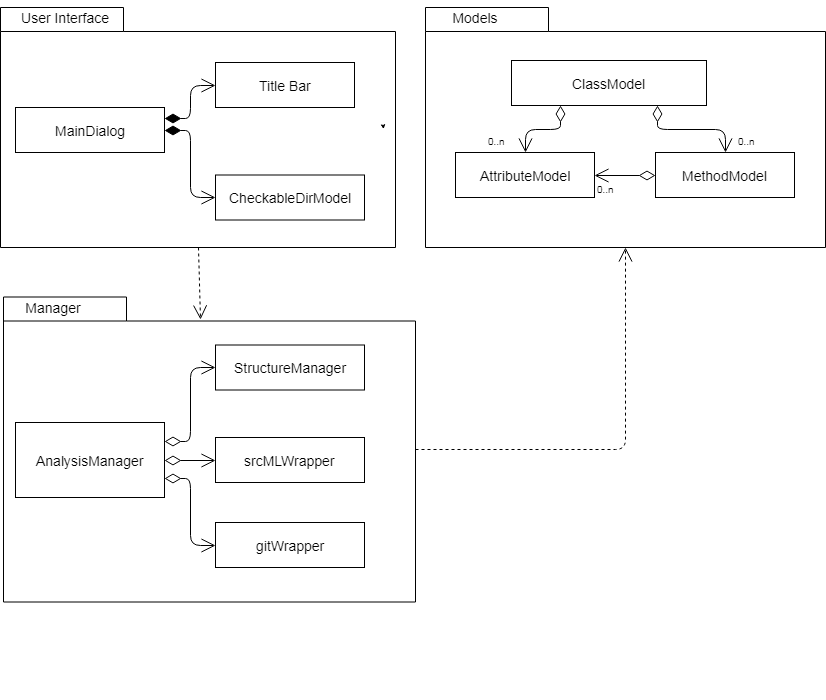
\includegraphics[width=\textwidth]{classdiagram.png}
\caption{UML diagram of the tool}
\label{fig:figdiagram}
\end{figure}

 \textit{\textbf{MainDialog}} is responsible for the User Interface creation . This class also handles the events from the user (process button pressed , load files button pressed, close window button pressed). MainDialog uses the TitleBar class for the title bar creation and CheckableDirModel for file system tree view. \\

The \textit{\textbf{ CheckableDirModel}} inherits QDirModel class which provides a data model for the local filesystem.In addition CheckableDirModel adds checkboxes to each filesystem item for a more easyer selection and returns a list of all files selected. \\

\textit{\textbf{ TitleBar}} inherits QMenuBar class which provides a horizontal menu bar. TitleBar class is used to create a new title bar, different from the one provided by Windows system . The class handles events like minimize , maximize and close window which are then emited to MainDialog class .\\

 A \textit{\textbf{ClassModel}} object contains all the informations extracted from the structural analysis about a class. ClassModel class contains a member for the name of the class , one for the parent name of the class and one for the xml file path in which the class was found. It also contains a list of MethodModels, a list of AttributeModels and 3 lists for git links, one for links found in commits with below 5 files changed , one for above 5 files changed and below 20 and one for links found in commits with above 20 files changed.The git links lists are lists of string objects. The class provides setters and getters for all the members mentioned above for retrieving and updating their values. \\

A \textit{\textbf{MethodModel}} object contains all the information extracted from the structural analysis about a method of a class. MethodModel contains a member for the name of the method and two lists of AttributeModels . One is used for the call parameters of the method and one is used for the local variables found inside the method.\\

 \textit{\textbf{AttributeModel}} contains two members , type and name. "Type" is used to identify the object type and "Name" is used to identify the object name. The class provides setters and getters for the members mentioned above for retrieving and updating their values. \\

 \textit{\textbf{AnalysisManager}} is created and called by  \textit{MainDialog}. MainDialog creates a AnalysisManager object and passes to it a list of source code files paths to be analysed and the parent folder path. The path to the parent folder is used to identify the Git repository. AnalysisManager is called each time the user triggers events in the User Interface. AnalysisManager calls the srcMLWrapper for XML conversion and XML files parsing and data extraction.\\ All the data extracted are passed to StructureManager. It also calls GitWrapper which interogates the project repository and saves all the commit differences in a temporary folder. The class is also responsable for parsing all the diff files and extracting the git links. The git links are passed to StructureManager which splits them into categories and setts them to the coresponding ClassModel object (figure \ref{fig:seq}). Finally is responsable for plotting the results of different queries (Example : all the overlappings between structural dependencies and logical dependencies extracted from commits with less then 5 files changed ) .\\

 \textit{\textbf{StructureManager}} contains all the ClassModels extracted  and is used by the AnalysisManager to save all datas extracted to an XML file and to load the datas extracted from an XML file (each project has an coresponding XML file that is created automaticaly after the analysis is done). Also is responsable to add the git links to the coresponding classes .\\

\textit{\textbf{srcMLWrapper}} has methods for converting source code files into XML files and to parse the resulting XML files in order to extract informations about classes , methods , members.\\

\textit{\textbf{GitWrapper}} identifies the git repository of the path given as a parameter and creates a temporary folder in which all the differences files are stored.


\begin{figure}
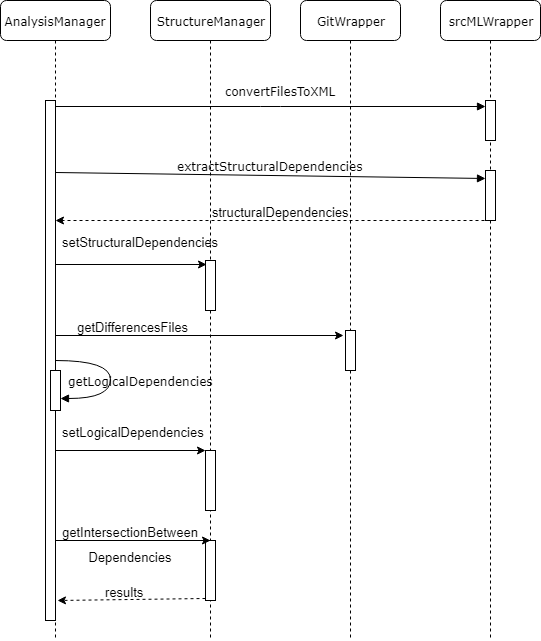
\includegraphics[scale=0.7]{flowdiag.png}
\caption{Sequence diagram}
\label{fig:seq}
\end{figure}

\section{User Interface}

\subsubsection{Creating MainDialog components}

MainDialog class inherits QMainWindow from PyQt which provides a main application window. The window is set as frameless window since a custom TitleBar will be attached to it. 

\begin{lstlisting}[language=python, caption={Create the title bar for the main window.}]
self.setWindowFlags(QtCore.Qt.FramelessWindowHint)
self.titleBar = TitleBar(self)
self.setMenuBar(self.titleBar)
\end{lstlisting}

In addition other widgets will be created : progress line , progress bar , tree view of the file system . All the above will be added after creation to the main layout of the window. There are two types of layouts in PyQt : \textit{QVBoxLayout} and \textit{QHBoxLayout} . The first layout lines up widgets vertically and the second horizontally.

\begin{lstlisting}[language=python, caption={Add widgets to the main window layout.}]
self.boxLayout = QVBoxLayout(self)

self.boxLayout.addWidget(self.tree)
self.boxLayout.addWidget(self.progressLine)
self.boxLayout.addWidget(self.progressBar)
\end{lstlisting}

\subsubsection{Creating Menus}
Qt implements menus in QMenu and QMainWindow keeps them in a QMenuBar. QAction is an abstraction for actions performed with a menubar and can be created with an icon and a name. After the creation, the action is connected to a method, so when we select a particular action, a triggered signal is emitted and the specified method executes. 

\begin{lstlisting}[language=python, caption={A menu creation with two actions.}]
processAction = QAction(QIcon('resources/run.png'), 'Process Files', self)
xmlLoadAction = QAction(QIcon('resources/load.png'), 'XML File', self)

processAction.triggered.connect(self.processFilesClicked)
xmlLoadAction.triggered.connect(self.loadXmlClicked)

self.toolbar.addAction(processAction)
self.toolbar.addAction(xmlLoadAction)
\end{lstlisting}

\section{Extracting software dependencies}
\subsection{srcML}
SrcML is an open source tool that converts in an XML format C/C\#/Cpp/Java source code. \cite{srcml1}\\
All the original source code files are kept and the corresponding XML files are created. Each source code file is converted in a single XML document.\\
 The srcML toolkit includes \textbf{source-to-srcML} and \textbf{srcML-to-source} translators:
\begin{itemize}
  \item source-to-srcML : is responsable for source code to XML conversion.
  \item srcML-to-source : is responsable for XML to source code conversion, so that the original source code document can be recreated from the srcML XML file.
\end{itemize}

The srcML XML contains of all text from the source code file and XML tags. The file contains all the syntactic structures from the code (e.g., classes, structures, functions, function call, destructors, methods, if statements, for statements, switch statements, etc.).\cite{srcml2}
An example of the XML representation can be found in Figure \ref{fig:figxml} .

\begin{figure*}[h]
\centering
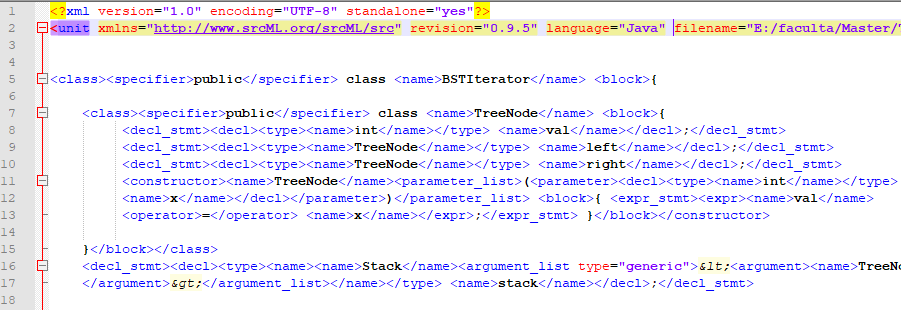
\includegraphics[width=\textwidth]{xmlscreenshot.PNG}
\caption{Example of XML representation of source code.}
\label{fig:figxml}
\end{figure*}

\subsection{Convert files to XML using srcML}
\tab As mentioned above, for conversion from source code to XML we will use srcML.
Through UI the user can choose the main folder of the to-be analysed project. The tool will walk trough all the subfolders and files of the folder and will get only the files that are source code files (files with extension such as .cpp ,.c++, .h , .java).
\begin{lstlisting}[language=python, caption={Walk through the given directory and extract only source code files}]
for path, dirs, files in os.walk(self.filePath(index)):
    for filename in files:
        if QtCore.QFileInfo(filename).completeSuffix() in acceptedSuffix:
             selection.add(os.path.join(path, filename))
\end{lstlisting}

The next step is to convert each file to XML. The conversion will be made through calls to srcML using the \textbf{subprocess} module . The subprocess module allows to spawn new processes, connect to their input/output/error pipes, and obtain their return codes. 
Arguments to pass to srcML :
\begin{itemize}
  \item the path to the file to-be-converted
  \item "-o" option , stands for outputting to a file 
  \item the output file path
\end{itemize}

\begin{lstlisting}[language=python, caption={Convert source code to XML using subprocess module.}]
def convertFiles(self, file):
    file_name = os.path.basename(file)
    file_xml = self.workingDir + "/"+file_name + ".xml"
     cmd = "srcml \""+file+"\" -o \""+file_xml+"\""
     rez = subprocess.Popen(cmd, shell=True, stdout=subprocess.PIPE).stdout.read()
\end{lstlisting}

\subsection{Extracting structural dependencies from XML}
\subsubsection{The ElementTree library}
For XML parsing we used \textbf{The ElementTree} library.It includes tools for parsing XML using event-based and document-based APIs, searching parsed documents with XPath expressions, and creating or modifying existing documents.
Parsing an entire document with parse() returns an ElementTree instance. The tree knows about all of the data in the input document, and the nodes of the tree can be searched or manipulated.

\begin{lstlisting}[language=python, caption={Import and create ElementTree instance}]
 import xml.etree.ElementTree as ET
 tree = ET.parse(file)
\end{lstlisting}

\subsubsection{Class extraction}
\textbf{Element.findall("name")} finds only elements with the tag "name" which are direct children of the current element. The items returned by findall() are Element objects, each representing a node in the XML tree. Each Element has attributes for accessing the data of the XML.
\begin{lstlisting}[language=python, caption={Get name of  Element item. }]
 def getName(self, item):
        if item is not None:
            text = item.text
            if text is None:
                return self.getText(item.find("name"))
            return text
\end{lstlisting}

\tab One xml file can contain one or more class types. Also one class can contain other class definitions so the parsing will be made recursively. Each time a new class is found a ClassModel object is created  and added to a list. 


\begin{lstlisting}[language=python, caption={Recursively find all the classes from XML file.}]
def getClassModelJava(self, file, root):
        classList = []

        for item in root.findall("{http://www.srcML.org/srcML/src}class"):
            className = self.getName(item)
            insideClassList = self.getClassModelJava(file, item)

            if insideClassList:
                classList.extend(insideClassList)

            classModel = ClassModel()
            classModel.setFile(file)
            classModel.setName(className)
		....
\end{lstlisting}

\subsubsection{Method extraction}
A ClassModel has a list of attributes and a list of methods. The methods are relevant because their call parameters and attributes can create structural dependencies. In order to get the parameters names we will look for \textbf{parameter\_list} tag inside the tree. For attributes we will look for \textbf{decl\_stmt} tag .
\begin{lstlisting}[language=python, caption={Get the parameter list of a method.}]
method = MethodModel()
method.setType(element_type)
method.setName(element_name)

for param in self.getAttributes(self.getItem(decl, "parameter_list"), "parameter"):
	method.addArgs(param)
....
classModel.addMethod(method)
\end{lstlisting}

\subsubsection{Attribute extraction}
Both ClassModel and MethodModel have a list of attributes.  Those attributes give the structural dependencies of the class . The call parameters of a function are also considered as attributes . We will refer to the AttributeModel class as a class that contain the information required to identify one side of the structural depencency link. The other side is the ClassModel containing the AttributeModel . 
\begin{lstlisting}[language=python, caption={Get the attributes list of a method or class.}]
for a in self.getAllItems(decl, "decl"):
   element_type = self.getType(a)
   element_name = self.getName(a)

   attribute = AttributeModel()
   attribute.setType(element_type)
   attribute.setName(element_name)

   attributes.append(attribute)
 return attributes
\end{lstlisting}

\section{Extracting logical dependencies}

\tab The second step of the analysis is to extract logical dependencies from the versioning system.  Changes can be made by many individuals over the years.\\ 
Changes include the creation and deletion of files as well as edits to their contents. Each change (this can include changes in multiple files) made by an individual at certain point of time is contained into a commit\cite{ct7}. \\ The tool looks through the repository and gets all the existing commits, for each commit a differences file will be made .After all the differences files are stored , all the files are parsed and logical dependencies are build. 

\subsection{Git repository configuration}
\label{ssec:gitrepo}
\tab To get informations about a git repository we use \textit{\textbf{GitPython}} library that provides object model access to the git repository. The first step is to create a git.Repo object to represent the repository, with the local repository path as argument. A repo object provides high-level access to the repository data and allows you to create and delete heads and access the configuration of the repository.\\
After the Repo object creation, the repository needs to be checked if it's bare or not .\\ A bare Git repository is typically used as a remote repository that is sharing a repository among several different people. The developers don't do work  inside the remote repository so there's no Working Tree (the project files that you edit), just bare repository data. If the repository is not bare then other configurations can be checked : repository description, active branch , number of commits.

\begin{lstlisting}[language=python, caption={Get informations about a git repository.}]
repo = Repo(self.repo_path)
if not repo.bare:
        print('Repo description: '.format(repo.description))
        print('Repo active branch is {}'.format(repo.active_branch))
        branches = repo.remotes.origin.refs
        print('Number of branches : {}'.format(len(branches)))
        for branch in branches:
            commits = list(repo.iter_commits(branch))
	  print('Branch named {} - commits number: {}'.format(branch, len(commits)))
\end{lstlisting}

\subsection{Get diff files of active branch}
\label{ssec:gitdiff}
\tab The tool iterates through all the commits from the active branch and creates the diff files. The differences file will contain all the changes from all the files merged. Each file will be saved with "\_FilesChanged\_" followed by the number of source code files changed in his name. In this way it will be more easy to extract the number of files changed and to filter the dependencies found by the number of files changed. \\ If a commit has 0 source code files changed then the commit will be ignored and no diff file will be created. The diff file will be created through a system call to git since GitPython does not have this functionality.
All the diff files will be saved in a temporary folder. 

\begin{lstlisting}[language=python, caption={Creating the diff files of the active branch commits.}]
commits = list(repo.iter_commits('master'))
index = 0
for commit in commits:
    parent = commit.parents[0] if commit.parents else EMPTY_TREE_SHA
    nrOfFilesChanged = self.getNrOfChangedFiles(commit, parent)
    if nrOfFilesChanged >= 1:
        os.system("git diff "+parent.hexsha+" "+commit.hexsha+" > "+self.repo_path+
"\~diffs\diff"+str(index)+"_FilesChanged_"+str(nrOfFilesChanged)+".txt")
        index += 1
\end{lstlisting}

\subsection{Get logical dependencies from diff files}
\tab All the actions mentioned in subsections \ref{ssec:gitrepo}  and \ref{ssec:gitdiff} are made by GitWrapper. The process of logical dependencies extraction from diff files is made by the AnalysisManager.\\
The first step in getting the logical dependencies from a diff file is to get the number of changed files.

\begin{lstlisting}[language=python, caption={Get number of changed files from file name.}]
file = file.replace('.txt', '')
nrOfCommitsStr = file.split('FilesChanged\_')[1]
nrOfCommits = int(nrOfCommitsStr)
\end{lstlisting}

The diff file can contain comments, in order to build logical dependencies without comments we need to call a function that removes all the comments from the diff file . The removing is made with the regular expressions library , re.
\begin{lstlisting}[language=python, caption={Remove comments from file.}]
def removeComments(self, filepath):
        string = open(filepath).read()
        string = re.sub(re.compile("/\*.*?\*/", re.DOTALL), "",string) 
        string = re.sub(re.compile("//.*?\n"), "", string)  
        return string
\end{lstlisting}

Next we need to identify the classes change. We will iterate through all the lines of the diff file and search for key words like "class" or "private class". If a line contains the keywords the the line will be split into words and the name of the class will be extracted.

\begin{lstlisting}[language=python, caption={Get classes changed from the diff file.}]
if re.search('.*class .*\{', line) or re.search('.* public class.*', line) 
or re.search('.* private class .*', line):
    words = line.split(' ')
    for i in range(0, len(words)):
         word = words[i].strip()
         if word == 'class' :
                   gitlist.append(words[i + 1].strip())
\end{lstlisting}

Finally, after the entire file is parsed and all the git links are gathered, we will add all the git links to the corresponding classes by calling \textit{setGitLinksToClass} method of the structure manager. For each class name found in the diff file all the other class names will be set as git links.
\begin{lstlisting}[language=python, caption={StructureManager call to set the git links.}]
if len(gitlist) > 1:
 for className in gitlist:
    self.structureManager.setGitDependenciesToClass(className, gitlist, nrOfCommits)
\end{lstlisting}

\subsection{Splitting git dependencies on categories}
\tab The following step after extracting all the git dependencies found in a diff file is to set the dependencies to the corresponding git classes .\\ For example, if in one diff file we found that classes A , B and C are updating together, then class A has logical dependencies with class B and C, Class B has logical dependencies with class A and B and Class C has logical dependencies with class A and B. \\ 
\tab One case often encountered is to found between the git dependencies list passed to the StructureManager some classes that are not known (their name is not among the classes held in StructureManager ). Since git dependencies are extracted from all the commits over time it can be posible that on class has been deleted or renamed meanwhile.\\ We will not take into consideration such cases since we only study the stability of the current state of the system . Structural dependencies are only identified from the source code of the last commit so we will only study the evolution of the classes found in it. So the classes that are not known will be ignored.

\begin{lstlisting}[language=python, caption={Set git dependencies to the coresponding classes.}]
def setGitDependenciesToClass(self, className, listOfDep, nrOfCommits):
   flag = False
     for classStruct in self.classlist:
        if classStruct.getName() == className:
            flag = True
            classStruct.setGitDependencies(listOfDep, nrOfCommits)
     if not flag:
            print("Class: " + className+" not found!")
\end{lstlisting}


\tab Each ClassModel has three lists for git dependencies (mentioned in this document also as links) . One for links found in diff files with less then 5 files changed, one for dependencies found in diff files with more then 5 and less then 20 files changed and one for dependencies found in diff files with more then 20 files changed .\\
\tab As mentioned in the previous section, ClassModel is responsible for dividing the dependencies received from  StructureManager, so as for each class in the received list all the other classes are set as logical dependencies.

\begin{lstlisting}[language=python, caption={Split dependencies in categories.}]
def setGitDependencies(self, dependencies, nrOfCommits):
   for dep in dependencies:
            if dep != self.name:
                if nrOfCommits <= 5:
                    self.git_dep_below5.append(dep)
                if 5 < nrOfCommits <= 20:
                    self.git_dep_below20.append(dep)
                if nrOfCommits > 20:
                    self.git_dep_more20.append(dep)
\end{lstlisting}

Because the entire list of git dependencies received from the AnalysisManager is passed to each ClassModel without taking out from the list the called class for which the other classes are set as logical dependencies, we will need to parse inside ClassModel the entire list and to make sure that the class is not added as logical dependencie to itself.

\section{Overlappings between logical and structural dependencies}

\subsubsection{Create unified list of structural dependencies for each class}
\tab Each ClassModel has a list of members and a list of methods . Each method contains also a lists of local variables and a list of call arguments . In order to build the lists with all the structural dependencies found in each class an additional list will be created in each ClassModel. The list will contain all the classes found in the members list of the class, call arguments, local variables of the methods and the superclass if exists.

\begin{lstlisting}[language=python, caption={Create unified list of structural dependencies.}]
self.relation_list = []
for attrib in self.attributes:
    self.relation_list.append(attrib.getType())
            
for method in self.methods:
   for arg in method.getArgs():
      self.relation_list.append(arg.getType())

for local in method.getLocals():
   self.relation_list.append(local.getType())

if self.superclass != "None":
   self.relation_list.append(self.superclass)

self.relation_list = [x for x in self.relation_list if x not in self.relation_list]
\end{lstlisting}

\tab The obtained list is filtered for duplicates. So the resulting list contains unique structural dependencies between the class and other classes. 

\subsubsection{Optain overlapings with logical dependencies}

\tab Once the structural dependencies list is build, we can find overlapping between the list and the structural dependencies lists.

\begin{lstlisting}[language=python, caption={Get overlapping between structural dependencies and logical dependencies found in diff files with less then 5 files changed.}]
def getMatch5(self):
        return set(self.relation_list).intersection(self.git_dep_below5)
\end{lstlisting}

\section{Saving and restoring the information processed}
\tab The process of saving all the informations about classes and structural and logical dependencies is made by StructureManager. The informations are saved in a single XML file, later the file can be loaded in the tool and by this a lot of time will be saved since it will be no need build the logical and structural dependencies from scratch.\\ For each member of the ClassModel , MethodModel and AttributeModel classes a xml tag is created. The XML file creation is made using ElementTree library. The Element class knows how to generate a serialized form of its contents, which can then be written to a file.\\ There are two functions used for creating a hierarchy of Element nodes. Element() creates a 
standard node and SubElement() attaches a new node to a parent.

\begin{lstlisting}[language=python, caption={Save informations to XML file using ElementTree.}]
def saveToXml(self):
    data = ET.Element('data')
    for classItem in self.classlist:
         classElement = ET.SubElement(data, 'class')
         className = ET.SubElement(classElement, 'name')
         className.text = classItem.getName()

         attribElement = ET.SubElement(classElement, 'attributes')
                for attribItem in classItem.getAttributes():
                    attrib = ET.SubElement(attribElement, 'attribute')
                    attribName = ET.SubElement(attrib, 'name')
                    attribName.text = attribItem.getName()

         gitLinksElement = ET.SubElement(classElement, 'gitlinksmore5below20')
         gitList = ",".join(gitLinksList)
         gitLinksElement.text = gitList

     filedata = ET.tostring(data)
     file = open(path, "w+")
     file.write(mydata)
\end{lstlisting}

\tab For the XML loading part , ElementTree is used again, the tool looks for tags like class , attribute, gitlinks and rebuilds all the structure with the collected informations.

\begin{lstlisting}[language=python, caption={Load informations from XML file using ElementTree.}]
tree = ET.parse(file)
root = tree.getroot()
for item in root.findall("class"):
   classModel = ClassModel()
   classModel.setFile(self.getItemTextByName(item, "file"))
   classModel.setName(self.getItemTextByName(item, "name"))
\end{lstlisting}

\section{Plots creation}
\tab After the logical and structural dependencies are extracted, a series of plots will be created by the tool . The plots are displayed by the tool but also saved as images in a results folder together with the generated XML file.\\
For plots creation \textbf{Matplotlib} and \textbf{NetworkX} is used. Matplotlib is a Python 2D plotting library and it provides an object-oriented API for embedding plots into applications using general-purpose GUI toolkits like Tkinter, wxPython, PyQt. 

\begin{lstlisting}[language=python, caption={Create plot with networkx.}]
 import matplotlib.pyplot as plt
plt.figure(1)
g = nx.Graph()
for classItem in self.structureManager.getClassList():
    g.add_node(classItem.name)
    related_list = classItem.getMatch()
    for related in related_list:
        g.add_edge(classItem.name, related)
       
plt.title("Code+ Git Links. Count: " + str(g.number_of_edges()))
\end{lstlisting}

\tab A Graph is a collection of nodes and pairs of nodes (called edges or links). In NetworkX, nodes can be any hashable object : a string, an image or an XML object. 
The graph creation is made by calling the Graph method of networkx. First, the class list held by StructureManager is parsed and nodes with the classes names are created. For each class a list of edges is build in function of the purpose of the graph .\\ For example if we build a graph with the overlappings between structural and all logical dependencies, we need to aquire for each class the list of coresponding logical dependencies list . The list will be parsed and edges will be created between the class and all the items of the list.
